
\chapter{绪论}\label{preface}

\section{研究背景}
无人驾驶飞机(Unmanned Aerial Vehicle)是无人飞行器的一种,简称无人机(UAV),它是由机体内部的飞行控制系统自主控制飞行任务,或者由飞机外控制器通过传送指令完成特定飞行任务的飞行器。飞行器内部无驾驶舱,但是由飞行动力装置,自动驾驶仪及程序控制装置组成。

随着科学技术的发展,无人机也能够完成以往只能由载人飞行器完成的任务,同时,无人机因其续航能力强,成本低廉,无人员伤亡等具备的载人飞行器不可比拟的优势,从而使无人机得到了广泛的应用。在军事方面,无人机除了可以完成电子干扰,对敌侦查,无线电中继等常规任务外,在危险恶劣的环境下,无人机还可以携带武器,例如:无人直升机不仅具备了直升机的共同优势,同时,因其垂直起降,自主悬停等独特的优点,无人直升机更适合在狭小的空间内进行飞行任务,在军事方面被广泛的应用在前沿阵地,舰船等狭窄的场地内起降,完成侦察敌情,勘测等任务\cite{yuyanping2010}。

在民用方面,无人机不仅可以应用到航拍技术,地形勘测,同时,还可以被用于抢险救灾,农业森林等方面。在很多载人飞行器无法直接操纵的环境中,无人机基于自身独特的优势,在地震抢险救灾,室内勘测等方面,常常担任空中机器人的角色。比如,新型的小型无人机因其成本低廉,结构简单,形状新颖,性能卓越以及独特的飞行控制方式\cite{liupeng2011},特别适合执行各种近地面环境的特殊任务。

\section{研究内容及论文结构}
本文研究目的是希望通过搭建飞行仿真平台,研究四旋翼无人机和固定翼无人机的飞行运动状态与姿态,从而提高飞行控制模型的鲁棒性。但是,现有的飞行仿真平台一般基于数值形态的计算,并不能够完全提供真实的三维视景仿真系统,从而不能够全面的反映出飞行控制系统的缺陷,具有一定的局限性。因此,本文基于开源的FlightGear飞行模拟软件,提供三维视景仿真系统,对飞机的飞行参数进行实时显示,同时,结合C++编程实现飞行摇杆设备对无人机飞行控制,直观真实的模拟飞行过程,有利于发现飞行控制系统的缺陷,从而使飞行仿真更加逼近真实的飞行情况。

在仿真平台搭建中,三维可视化的研究是非常重要的环节,可以对无人机的运动状态及总体结构进行直观显示\cite{lihaiquan2011},从而实现实时显示无人机的飞行位置及姿态变化的效果,增加飞行仿真的真实性。飞行仿真实验平台对飞行器测试研究工作有重要的作用,不仅可以总结飞机的飞行规律,而且能够对飞机的性能进行评估,从而降低试飞的风险和成本,提高飞行的安全性。

基于以上内容,本文的论文结构主要由六部分组成,如图\ref{fig1}所示。
\vspace{10pt}
\begin{figure}[!ht]
\centering
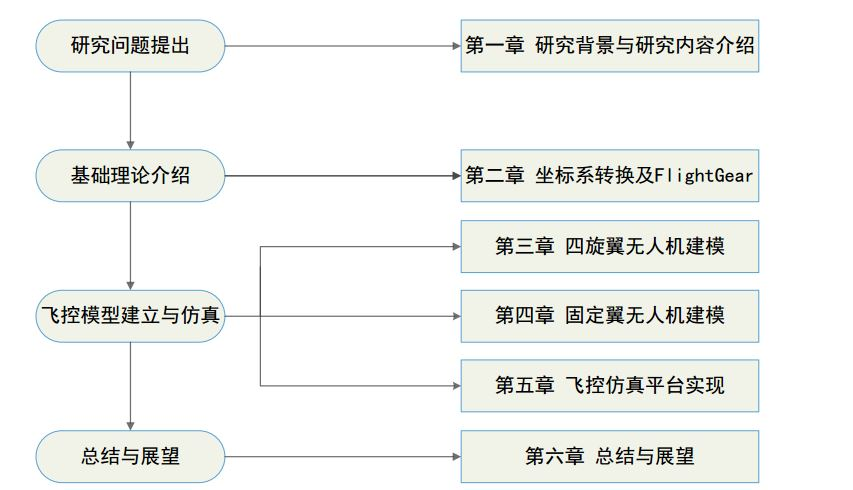
\includegraphics[width=0.8\textwidth]{f1.jpg}
\caption{论文结构 }
\label{fig1}
\end{figure}


第\ref{preface}章:主要介绍问题提出的研究背景,研究内容及研究目的,从宏观的角度对本文进行概括,对问题进行概述。

第\ref{introduction}章:推导四旋翼无人机坐标系变换公式与介绍FlightGear软件基础,概述FlightGear 软件的运作流程。

第\ref{conclusion}章:总结建模过程中的创新点与改进之处,提出进一步研究的方向与进度,对未来的研究工作提出展望。

